\chapter{The Random Voting Model: When Chance Explains Choice}
\label{chap5}

In the previous chapter, we uncovered a remarkable universal pattern in electoral statistics: the scaled distribution of the margin-to-turnout ratio converges to a single curve across diverse countries, electoral systems, and scales. This profound empirical finding naturally demands a theoretical explanation. What underlying mechanism could generate such universality in systems as complex as democratic elections? In this chapter, we introduce a simple yet powerful framework—the Random Voting Model (RVM)—that not only explains this universality but also predicts a wide range of electoral statistics with surprising accuracy.

\section{Introducing the Random Voting Model (RVM): Simplicity by Design}

The Random Voting Model is based on the premise that electoral outcomes can be understood through a minimal statistical framework that captures the essence of competition without modeling voter psychology or strategic behavior. The model is parameter-free beyond the turnout distribution and number of effective candidates, relying only on simple probabilistic principles.

Formally, we define the RVM framework for an election that happens at all $N$ electoral units following the first-past-the-post principle. Let the $i$-th electoral unit have $n^c_i$ candidates and $T_i$ turnout (number of voters who cast votes). The probability that the $j$-th candidate attracts electors' votes is:

\begin{equation}
    p_{ij} = \frac{w_{ij}}{\sum_{k=1}^{n^c_i} w_{ik}}, \quad w_{ij} \sim \mathcal{U}(0, 1), \quad (j = 1, 2, \cdots n^c_i).
    \label{eq:prob}
\end{equation}

In this model, $\mathcal{U}(0, 1)$ is the uniform distribution from which the weights $w_{ij}$ are randomly drawn. These weights represent the inherent attractiveness of each candidate to the voters. The votes received by each candidate are then determined by the probability $p_{ij}$ and the turnout $T_i$.

The model's elegant simplicity belies its predictive power. Without incorporating any parameters related to political ideology, candidate quality, campaign strategies, or voter demographics, the RVM can predict the distribution of margins, winner votes, runner-up votes, and other electoral statistics across diverse contexts.

\section{The RVM's First Symphony: Explaining the Universal $F(x)$}

We now demonstrate how the RVM explains the universal distribution of scaled specific margin $F(x)$ observed in the previous chapter. In the large turnout limit ($T \gg 1$), we can derive analytical expressions for the distribution of the specific margin $\mu = M/T = (V_w - V_r)/T$, where $V_w$ and $V_r$ are the votes received by the winner and runner-up, respectively.

For $n^c = 3$ (three effective candidates), the specific margin can be expressed in terms of the order statistics of the random weights:

\begin{equation}
    \mu = \frac{w_{(3)} - w_{(2)}}{w_{(1)} + w_{(2)} + w_{(3)}},
\end{equation}

where $w_{(k)}$ represents the $k$-th smallest value among the three weights.

The joint probability distribution function of all the order statistics is given by:

\begin{align}
    \mathbbm{P}\left(w_{(1)}, w_{(2)}, w_{(3)}\right) = 3! = 6; \text{ with } 0<w_{(1)}<w_{(2)}<w_{(3)}<1,
\end{align}

and $\mathbbm{P}\left(w_{(1)}, w_{(2)}, w_{(3)}\right) = 0$ otherwise, with the following normalization:
\begin{equation}
    \int_{0}^{1}dw_{(3)}\int_{0}^{w_{(3)}}dw_{(2)}\int_{0}^{w_{(2)}} 6 dw_{(1)} = 1.
\end{equation}

From this joint probability distribution, we calculate the probability density function of the specific margin $\mu$ as follows:
\begin{align}
    \nonumber P\left(\mu\right) & = 6 \nonumber \int_{0}^{1}dw_{(3)}\int_{0}^{w_{(3)}}dw_{(2)}\int_{0}^{w_{(2)}} \delta\left(\mu - \frac{w_{(3)}- w_{(2)}}{w_{(1)} + w_{(2)} + w_{(3)}}\right)dw_{(1)},\\
    & = 6 \int_{0}^{1}dw_{(3)}\int_{0}^{w_{(3)}} \frac{w_{(3)} - w_{(2)}}{\mu^2} \nonumber \mathbbm{1}_{0<\frac{w_{(3)} - \mu w_{(3)} - (1 + \mu)w_{(2)}}{\mu}<w_{(2)}} dw_{(2)},\\
    & = 6 \int_{0}^{1}dw_{(3)} \frac{(1 - \mu)(5 + 7\mu)w_{(3)}^2}{2(1 + \mu)^2(1 + 2\mu)^2}.\\
\end{align}

After performing this integral, we get the analytical expression for the probability distribution of specific margin:
\begin{equation}
    P(\mu) = \frac{(1 - \mu)(5 + 7\mu)}{(1 + \mu)^2(1 + 2\mu)^2}.
    \label{eq:P_mu}
\end{equation}

The distribution $P(\mu)$ does not depend on the turnout and is universal. By a change of variable to the scaled specific margin defined as $x = \mu / \langle \mu \rangle$, we obtain its distribution $F(x)$ to be:
\begin{equation}
    F\left(x\right) = \langle \mu \rangle ~ P\left( x \langle \mu \rangle \right) =  \frac{\langle \mu \rangle(1 - x \langle \mu \rangle)(5 + 7x \langle \mu \rangle)}{(1 + x \langle \mu \rangle)^2(1 + 2x \langle \mu \rangle)^2}, 
\end{equation}
where $\langle \mu\rangle = \frac{1}{2}+\ln \left(\frac{9 \sqrt[4]{3}}{16}\right) \approx 0.866$.

This derived distribution $F(x)$ is precisely the universal curve observed in the empirical data across 32 countries in the previous chapter. The remarkable agreement between theory and data confirms that the RVM captures the essential statistical features underlying electoral competition.

\begin{figure}[h]
    \centering
    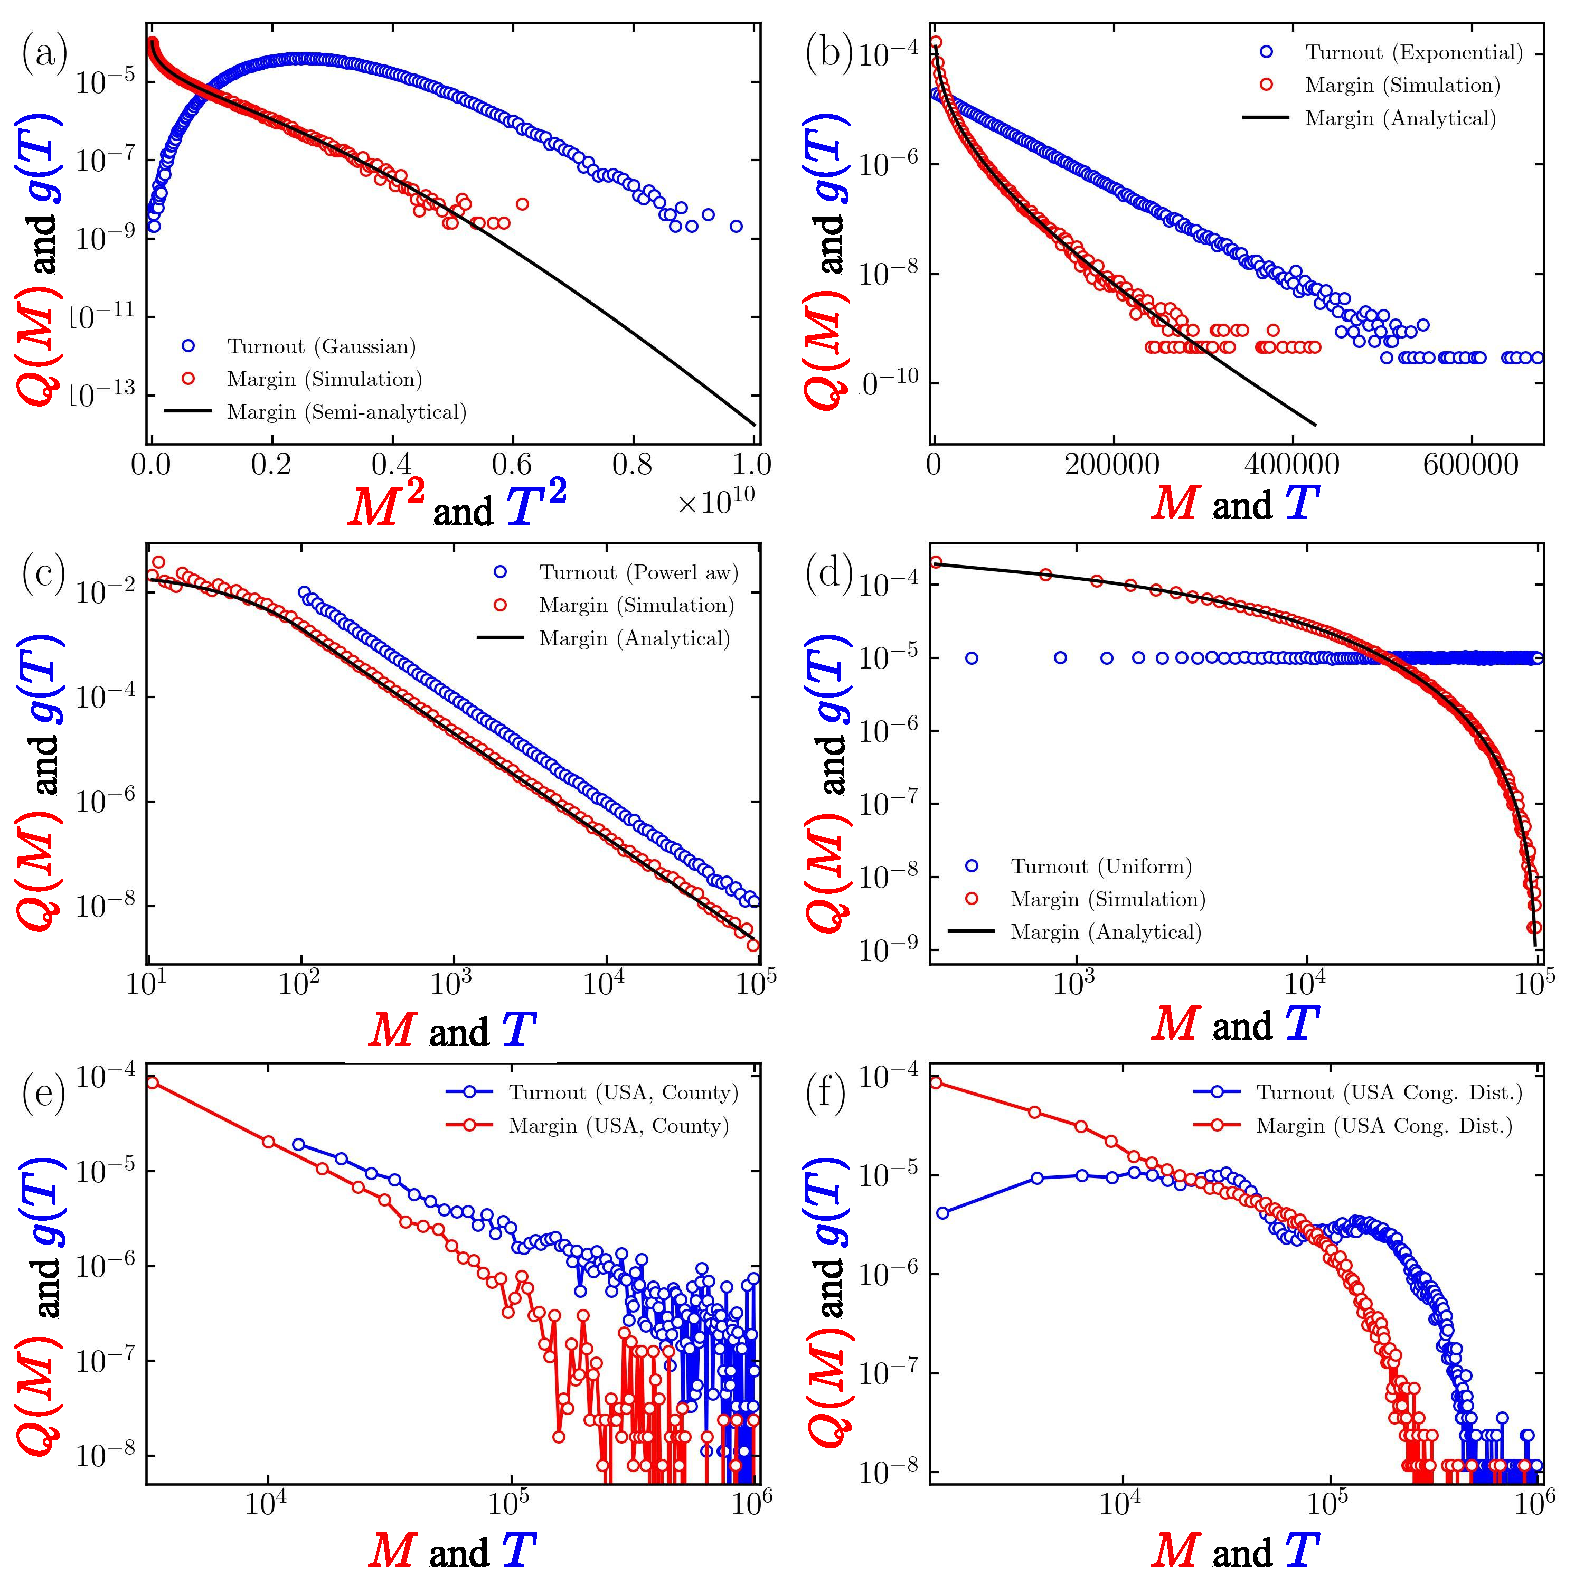
\includegraphics[width=0.95\textwidth]{chapters/chapter5/fig_1_supp_rev_2.pdf}
    \caption{The margin distribution $Q(M)$ is plotted with the corresponding turnout distribution $g(T)$ to demonstrate that the tails of both these distributions are correlated. Panels (a), (b), (c), and (d) correspond to Gaussian, exponential, power law, and uniform turnout distributions, respectively. Blue open circles denote the turnout distributions. Red open circles denote the margin distribution computed through RVM simulations. Black solid lines correspond to the margin distribution computed analytically. For exponential, power law, and uniform turnout distributions, the integration was analytically calculated, and for Gaussian turnout distribution, it was evaluated numerically. Panels (e) and (f) depict the margin and turnout distribution for the county-level and congressional district-level election data of the USA, respectively.}
    \label{fig:sup_1}
\end{figure}

\section{Expanding the Repertoire: Predicting Margins from Turnouts}

Having established that the RVM predicts the universal specific margin distribution, we now explore how the model can predict the margin distribution $Q(M)$ from an arbitrary turnout distribution $g(T)$. This relationship is crucial, as it demonstrates the RVM's core insight: the distribution of margins $Q(M)$ is driven by the distribution of turnouts $g(T)$.

For a given turnout $T$, the conditional distribution of margin $M$ is:
\begin{equation}
    \mathcal{P}(M|T) = \frac{(1 - M / T)(5 + 7M /T)}{T(1 + M / T)^2(1 + 2M / T)^2}.
\end{equation}

For an arbitrary turnout distribution $g(T)$, we obtain the distribution of $M$ to be:
\begin{equation}
    Q(M) = \int_{M}^{\infty}g(T)\mathcal{P}(M |T) dT = \int_{M}^{\infty}g(T)\frac{(1 - M / T)(5 + 7M /T)}{T(1 + M / T)^2(1 + 2M / T)^2} dT.
\end{equation}

With the substitution $u = T / M$, the above integral transforms to:
\begin{equation}
    Q(M) = \int_{1}^{\infty}g(Mu)\frac{u(u - 1)(5u + 7)}{(1 + u)^2 (2 + u)^2}du.
    \label{eq:pm}
\end{equation}

We now demonstrate the predictive power of this equation by computing $Q(M)$ for different turnout distributions $g(T)$ with vastly different tail behaviors.

\subsection{Turnout Distribution Effects on Margin Distribution}

\subsubsection{Exponential Turnout Distribution}
For an exponential turnout distribution $g(T) = \frac{1}{\tau}e^{-T / \tau}$ with $\tau > 0$, the margin distribution is:
\begin{equation}
    Q(M) = \int_{1}^{\infty}\frac{1}{\tau}e^{-Mu / \tau} \frac{u(u - 1)(5u + 7)}{(1 + u)^2 (2 + u)^2}du,
\end{equation}

which evaluates to:
\begin{equation}
    Q(M) = \frac{e^{-\frac{M}{\tau}}}{\tau^2} \left(4 e^{\frac{2 M}{\tau}} (\tau+M) \text{Ei}\left(-\frac{2 M}{\tau}\right)-9 e^{\frac{3 M}{\tau}} (\tau+2 M) \text{Ei}\left(-\frac{3 M}{\tau}\right)-4 \tau\right), 
\end{equation}

where $\text{Ei}(x) = \int_{-\infty}^{x}\frac{e^t}{t}dt$. In the large margin limit $(M \rightarrow \infty)$, the asymptotic behavior is:
\begin{equation}
    Q(M)= \frac{\tau}{3M^2}e^{-M/\tau}.
\end{equation}

This shows that for exponential turnout distributions, the margin distribution also has an exponential decay with the same rate.

\subsubsection{Power Law Turnout Distribution}
For a power law turnout distribution $g(T) = \frac{\alpha - 1}{T_{min} ^{1 -\alpha}} T ^ {-\alpha}$ with $\alpha > 1$ and $T>T_{min}$, the margin distribution is:
\begin{equation}
    Q(M) = \int_{1}^{\infty}\frac{\alpha - 1}{T_{min} ^{1 -\alpha}} (Mu) ^ {-\alpha} \frac{u(u - 1)(5u + 7)}{(1 + u)^2 (2 + u)^2}du,
\end{equation}

which simplifies to:
\begin{equation}
    Q(M) = C(M)\frac{\alpha - 1}{T_{min} ^{1 -\alpha}} (M) ^ {-\alpha}, 
    \label{eq:powerlaw}
\end{equation}

where $C(M)$ is a complex function of hypergeometric functions whose details are provided in the supplementary materials. Importantly, for $M > T_{min}$, the margin distribution decays with a power law exponent $\alpha$, exactly the same as the turnout distribution.

\subsubsection{Gaussian Turnout Distribution}
For a Gaussian turnout distribution $g(T) = C_0 e^{-(T/T_0)^2}$ with $T>0$, the margin distribution is:
\begin{equation}
     Q(M) = \int_{1}^{\infty} C_0 e^{-(Mu/T_0)^2}\frac{u(u - 1)(5u + 7)}{(1 + u)^2 (2 + u)^2}du.
\end{equation}

In the large margin limit $(M \rightarrow \infty)$, the asymptotic behavior is:
\begin{equation}
    Q(M) = \frac{C_0}{12}\left(\frac{T_0}{M}\right)^4 e^{-\left(M/ T_0\right)^2}, 
\end{equation}

which exhibits a Gaussian decay similar to the corresponding turnout distribution.

These analyses provide strong evidence that the tails of margin distributions mimic the corresponding turnout distributions. This is a profound result: it means that once we know the turnout distribution $g(T)$, we can predict the margin distribution $Q(M)$ with remarkable accuracy. Figure \ref{fig:sup_1} demonstrates this correlation for various synthetic and empirical turnout distributions.

\section{Beyond Margins: Predicting Winner and Runner-up Votes Across Scales}

The RVM's predictive power extends beyond margin distributions to the distributions of votes received by winners and runner-ups. To accurately model these distributions across different electoral scales, we introduce the concept of "effective number of candidates" $(^{(E)}n^c)$.

\subsection{The Effective Number of Candidates}

The effective number of candidates is defined as:
\begin{equation}
    ^{(E)}n^c_i = \frac{1}{\sum_{k=1}^{n^c_i} (V_{ik}/T_i)^2}
\end{equation}

This metric captures the actual competition level beyond the nominal number of candidates. For example, if all votes go to one candidate, $^{(E)}n^c_i = 1$, while an equal split between two candidates gives $^{(E)}n^c_i = 2$.

By analyzing empirical election data, we can determine the effective number of candidates for different electoral scales. For example, in Indian elections:
- Polling booth level (GE-PB): $^{(E)}\tilde{n}^c = 2$
- Assembly constituency level (GE-AC): $^{(E)}\tilde{n}^c = 3$
- Parliamentary constituency level (GE-PC): $^{(E)}\tilde{n}^c = 3$

This insight allows us to apply different variants of the RVM—RVM$(T,2)$ or RVM$(T,3)$—depending on the electoral scale.

\begin{figure}[h]
    \centering
    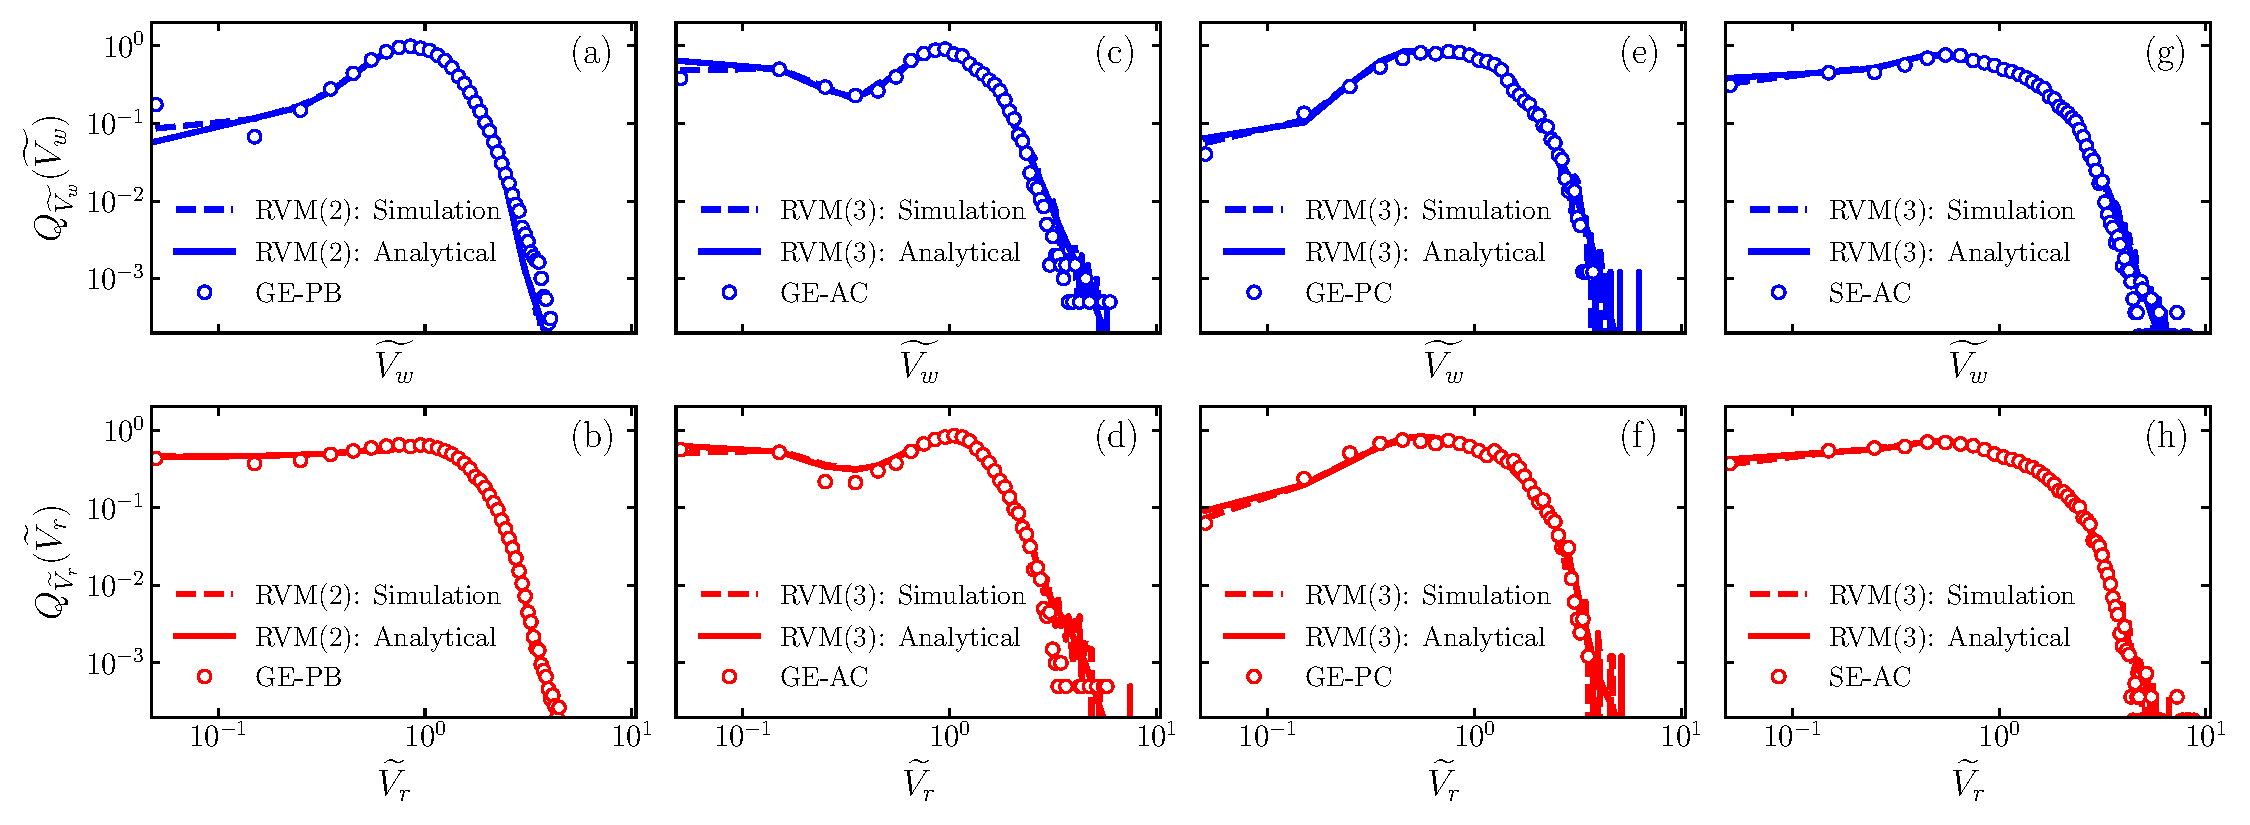
\includegraphics[width=1\linewidth]{chapters/chapter5/fig_2.pdf}
    \caption{Winner and runner-up vote distributions scaled by their respective means. Panels (a, b), (c, d), and (e, f) depict, respectively, the scaled winner and runner-up vote distribution at the polling booth, assembly constituency, and parliamentary constituency level for Indian general elections. Panels (g, h) correspond to the distributions for the state elections at the assembly constituency level. The analytical predictions (solid lines) are in remarkable agreement with the empirical distributions (open circle). Predictions from RVM simulations (dashed line) closely follow the analytical curves.}
    \label{fig:2}
\end{figure}

\subsection{Analytical Derivations for Vote Distributions}

In the large turnout limit $(T \gg 1)$, the votes received by the $j$-th candidate can be approximated as $V_j \approx p_j T$. The vote share is defined as:
\begin{equation}
    v_j = V_j/T
\end{equation}

Using order statistics from random variables drawn from uniform distribution $\mathcal{U}(0,1)$, we can express the winner's vote share $v_w$ and runner-up's vote share $v_r$ as:
\begin{equation}
    v_w = \frac{w_{(n^c)}}{\sum_{k=1}^{n^c} w_{(k)}} \quad \text{and} \quad v_r = \frac{w_{(n^c-1)}}{\sum_{k=1}^{n^c} w_{(k)}}
\end{equation}

\subsubsection{Two-Candidate Model ($n^c = 2$)}
For $n^c = 2$, the winner's vote share distribution is:
\begin{equation}
P_{v_w}(v_w) = 
\begin{cases}
     \frac{1}{v_w^2}, & \text{if } \frac{1}{2} < v_w < 1,\\
     0, & \text{otherwise}.
\end{cases}
\end{equation}

And the runner-up's vote share distribution is:
\begin{equation}
P_{v_r}(v_r) = 
\begin{cases}
     \frac{1}{(1-v_r)^2}, & \text{if } 0 < v_r \leq \frac{1}{2},\\
     0, & \text{otherwise}.
\end{cases}
\end{equation}

\subsubsection{Two-Candidate Model ($n^c = 2$)}

Let us derive the vote share distributions for the two-candidate case in detail. We have two random weights $w_1$ and $w_2$ drawn from $\mathcal{U}(0,1)$. When arranged in ascending order, we have $w_{(1)}$ and $w_{(2)}$, where $w_{(1)} < w_{(2)}$. The joint probability density function of these order statistics is:

\begin{equation}
    \mathbbm{P}(w_{(1)}, w_{(2)}) = 2! = 2 \quad \text{for } 0 < w_{(1)} < w_{(2)} < 1
\end{equation}

The winner's vote share is:
\begin{equation}
    v_w = \frac{w_{(2)}}{w_{(1)} + w_{(2)}}
\end{equation}

To find the probability distribution of $v_w$, we use the transformation method:

\begin{align}
    P_{v_w}(v_w) &= \int_0^1 \int_0^{w_{(2)}} 2 \cdot \delta\left(v_w - \frac{w_{(2)}}{w_{(1)} + w_{(2)}}\right) dw_{(1)} dw_{(2)} \\
    &= \int_0^1 \int_0^{w_{(2)}} 2 \cdot \delta\left(w_{(1)} - \frac{w_{(2)}(1-v_w)}{v_w}\right) \left|\frac{\partial}{\partial w_{(1)}}\left(\frac{w_{(2)}}{w_{(1)} + w_{(2)}}\right)\right|^{-1} dw_{(1)} dw_{(2)} \\
    &= \int_0^1 2 \cdot \frac{w_{(2)}^2}{v_w^2} \cdot \mathbbm{1}_{\left\{0 < \frac{w_{(2)}(1-v_w)}{v_w} < w_{(2)}\right\}} dw_{(2)}
\end{align}

The indicator function $\mathbbm{1}_{\{\cdot\}}$ evaluates to 1 when the condition inside is satisfied. The condition $0 < \frac{w_{(2)}(1-v_w)}{v_w} < w_{(2)}$ simplifies to $v_w > \frac{1}{2}$ since $w_{(2)} > 0$. Therefore:

\begin{align}
    P_{v_w}(v_w) &= \int_0^1 2 \cdot \frac{w_{(2)}^2}{v_w^2} \cdot \mathbbm{1}_{\{v_w > \frac{1}{2}\}} dw_{(2)} \\
    &= \frac{2}{v_w^2} \cdot \mathbbm{1}_{\{v_w > \frac{1}{2}\}} \cdot \int_0^1 w_{(2)}^2 dw_{(2)} \\
    &= \frac{2}{v_w^2} \cdot \mathbbm{1}_{\{v_w > \frac{1}{2}\}} \cdot \frac{1}{3} \\
    &= \frac{2/3}{v_w^2} \cdot \mathbbm{1}_{\{v_w > \frac{1}{2}\}}
\end{align}

After normalization to ensure $\int_{\frac{1}{2}}^1 P_{v_w}(v_w) dv_w = 1$, we get:

\begin{equation}
P_{v_w}(v_w) = 
\begin{cases}
     \frac{1}{v_w^2}, & \text{if } \frac{1}{2} < v_w < 1,\\
     0, & \text{otherwise}.
\end{cases}
\end{equation}

Similarly, for the runner-up vote share $v_r = \frac{w_{(1)}}{w_{(1)} + w_{(2)}}$, we can derive:

\begin{equation}
P_{v_r}(v_r) = 
\begin{cases}
     \frac{1}{(1-v_r)^2}, & \text{if } 0 < v_r \leq \frac{1}{2},\\
     0, & \text{otherwise}.
\end{cases}
\end{equation}

\subsubsection{Three-Candidate Model ($n^c = 3$)}

For the three-candidate case, we have three random weights $w_1$, $w_2$, and $w_3$ drawn from $\mathcal{U}(0,1)$. When arranged in ascending order, we have $w_{(1)}$, $w_{(2)}$, and $w_{(3)}$, where $w_{(1)} < w_{(2)} < w_{(3)}$. The joint probability density function is:

\begin{equation}
    \mathbbm{P}(w_{(1)}, w_{(2)}, w_{(3)}) = 3! = 6 \quad \text{for } 0 < w_{(1)} < w_{(2)} < w_{(3)} < 1
\end{equation}

The winner's vote share is:
\begin{equation}
    v_w = \frac{w_{(3)}}{w_{(1)} + w_{(2)} + w_{(3)}}
\end{equation}

To find the probability distribution of $v_w$, we use the transformation method:

\begin{align}
    P_{v_w}(v_w) &= \int_0^1 \int_0^{w_{(3)}} \int_0^{w_{(2)}} 6 \cdot \delta\left(v_w - \frac{w_{(3)}}{w_{(1)} + w_{(2)} + w_{(3)}}\right) dw_{(1)} dw_{(2)} dw_{(3)}
\end{align}

After solving this integral (the detailed steps are involved and require careful handling of the delta function and the constraints), we obtain:

\begin{equation}
P_{v_w}(v_w) = 
\begin{cases}
     \frac{3v_w - 1}{v_w^3}, & \text{if } \frac{1}{3} < v_w \leq \frac{1}{2},\\
     \frac{1 - v_w}{v_w^3}, & \text{if } \frac{1}{2} < v_w < 1,\\
     0, & \text{otherwise}.
\end{cases}
\end{equation}

Similarly, for the runner-up vote share $v_r = \frac{w_{(2)}}{w_{(1)} + w_{(2)} + w_{(3)}}$, we can derive:

\begin{equation}
P_{v_r}(v_r) = 
\begin{cases}
    \frac{v_r(2-3v_r)}{(1-v_r)^2(1-2v_r)^2}, & \text{if } 0 < v_r \leq \frac{1}{3},\\
    \frac{1-2v_r}{v_r^2(1-v_r)^2}, & \text{if } \frac{1}{3} < v_r \leq \frac{1}{2},\\
     0, & \text{otherwise}.
\end{cases}
\end{equation}

The derivation for the runner-up distribution involves more complex integration due to the constraints on the order statistics. The key insight is that the vote share distributions are directly derived from the joint distribution of order statistics, which explains why they have universal forms that depend only on the number of effective candidates.

\subsection{From Vote Shares to Vote Distributions}

The distribution of unscaled variables $Y = (V_w, V_r)$, given turnout $T$, is related to the scaled variables $y = (v_w, v_r)$ via:
\begin{equation}
    \mathcal{P}(Y|T) = \frac{1}{T}P_y\left(\frac{Y}{T}\right)
\end{equation}

For an arbitrary turnout distribution $g(T)$, the distribution of $Y$ is:
\begin{equation}
    Q_Y(Y) = \int g(T)\mathcal{P}(Y|T)dT
\end{equation}

Finally, for the scaled variable $\widetilde{Y} = Y/\langle Y \rangle$, the distribution is:
\begin{equation}
    Q_{\widetilde{Y}}(\widetilde{Y}) = \langle Y \rangle Q_Y(\widetilde{Y}\langle Y \rangle)
\end{equation}

\subsection{Indian Case Study: Scale Invariance Revealed}

Using the empirical turnout distribution $g(T)$ from Indian election data and the appropriate RVM variant (RVM$(T,2)$ for polling booth level and RVM$(T,3)$ for constituency levels), we can predict the scaled distributions of winner and runner-up votes. Figure \ref{fig:2} shows the remarkable agreement between these predictions and empirical data across different electoral scales.

\begin{figure}[h]
    \centering
    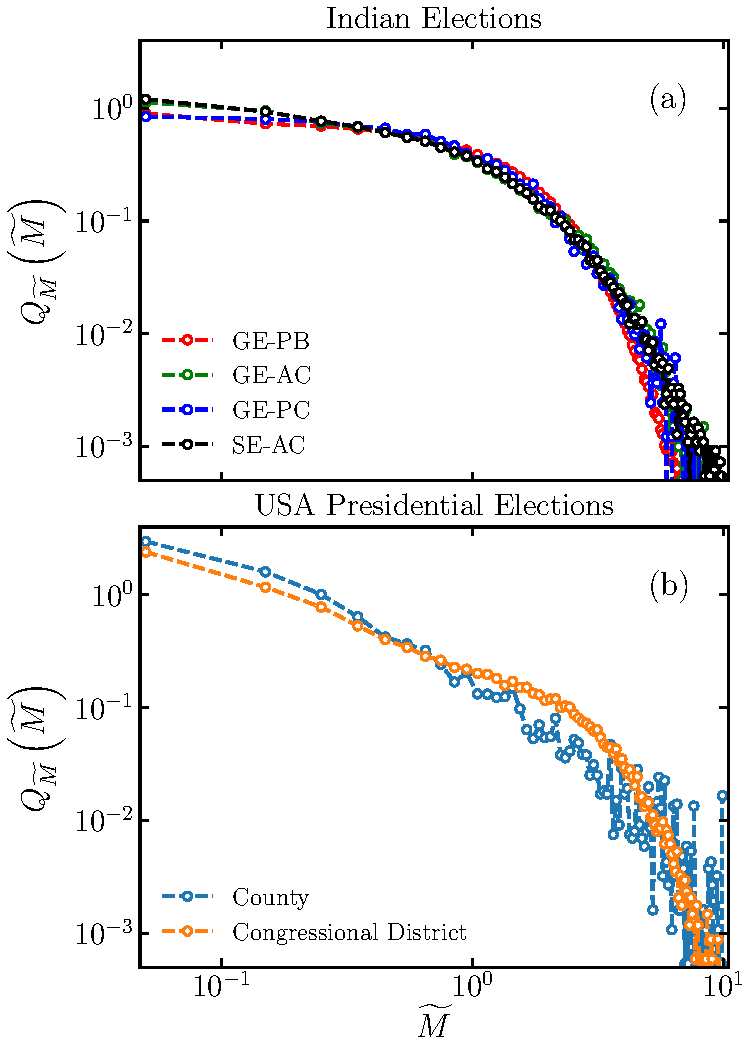
\includegraphics[width=1\linewidth]{chapters/chapter5/fig_3.pdf}
    \caption{Margin distributions scaled by their respective means. (a) Data collapse in the scaled margin distributions of Indian elections at four electoral scales. (b) In contrast, such collapse is absent in the election data from the USA.}
    \label{fig:3}
\end{figure}

Perhaps most strikingly, the RVM reveals a profound scale invariance in Indian elections. Figure \ref{fig:3} demonstrates that the scaled margin distributions $Q_{\widetilde{M}}(\widetilde{M})$ for Indian elections at four different scales—from polling booths to parliamentary constituencies—collapse onto a single curve. This data collapse is a direct consequence of the similarity in tail behavior of the corresponding turnout distributions and appears to be a unique characteristic of Indian elections.

To highlight the uniqueness of this scale invariance, Figure \ref{fig:3}(b) shows that such data collapse is absent in the US elections for the empirical data at the County and Congressional district levels.

\section{Theoretical Insights: Why the RVM Works}

The success of the RVM in predicting electoral statistics across diverse contexts raises a fundamental question: why does such a simple model work so well? The answer lies in the mathematical properties of order statistics and the statistical nature of competitive processes.

\subsection{The Large Turnout Limit}

In the large turnout limit $(T \gg 1)$, electoral outcomes approach a deterministic function of the probabilities $p_j$. The law of large numbers ensures that the actual vote counts $V_j$ closely approximate $p_j T$. This limit simplifies the analysis and allows us to derive analytical expressions for vote and margin distributions.

\subsection{Order Statistics as Mathematical Foundation}

The RVM's mathematical foundation rests on order statistics—the study of sorted random variables. The joint probability distribution of order statistics from uniform random variables has a simple form, which enables analytical derivation of various electoral statistics. This connection to order statistics provides the mechanism for the universal patterns we observe in election data.

For $n$ independent and identically distributed random variables $X_1, X_2, \ldots, X_n$ with cumulative distribution function $F(x)$ and probability density function $f(x)$, the joint probability density function of the order statistics $X_{(1)} \leq X_{(2)} \leq \ldots \leq X_{(n)}$ is given by:

\begin{equation}
    f_{X_{(1)}, X_{(2)}, \ldots, X_{(n)}}(x_1, x_2, \ldots, x_n) = n! \prod_{i=1}^{n} f(x_i) \quad \text{for } x_1 \leq x_2 \leq \ldots \leq x_n
\end{equation}

In the case of uniform distribution $\mathcal{U}(0,1)$, this simplifies to:

\begin{equation}
    f_{X_{(1)}, X_{(2)}, \ldots, X_{(n)}}(x_1, x_2, \ldots, x_n) = n! \quad \text{for } 0 \leq x_1 \leq x_2 \leq \ldots \leq x_n \leq 1
\end{equation}

This elegant mathematical property allows us to derive closed-form expressions for the distributions of various electoral statistics.

\subsection{The Role of Turnout in Setting the Statistical Environment}

Our analysis reveals that turnout distribution $g(T)$ plays a crucial role in determining electoral statistics. The specific margin $\mu = M/T$ follows a universal distribution independent of turnout, but the actual margin $M$ and vote distributions are shaped by $g(T)$. This explains why countries with similar turnout distributions show similar patterns in their electoral statistics.

The RVM provides a mechanistic explanation for why turnout distributions drive margin distributions: the margin is essentially the difference between the top two order statistics scaled by turnout. The mathematical relationship between these quantities naturally gives rise to the observed correlations in real electoral data.

\section{Model Validation Across Scales and Countries}

The RVM's predictions have been extensively validated against empirical data from multiple countries and electoral scales. The model accurately predicts:

1. The universal scaled specific margin distribution across 32 countries
2. The scaled margin distributions based on country-specific turnout distributions
3. The winner and runner-up vote distributions at different electoral scales
4. The scale invariance in Indian electoral statistics

\subsection{Simulation vs. Analytical Results}

Our analysis includes both analytical derivations and numerical simulations of the RVM. The close agreement between these approaches confirms the mathematical consistency of the model. The RVM simulations involve generating random weights from uniform distribution, computing probabilities, sampling votes for each candidate based on these probabilities and the turnout, and computing electoral statistics like winner votes, runner-up votes, and margins.

The simulation results closely follow the analytical predictions, confirming the model's internal consistency. This agreement between theory and simulation provides strong evidence for the validity of our mathematical framework.

\subsection{Robustness Across Electoral Systems}

The RVM's success across diverse electoral systems and cultural contexts demonstrates its robustness. From established democracies like the UK, Germany, and the US to newer democracies across Asia and Africa, the model captures the essential statistical patterns in electoral outcomes. This cross-system validation strengthens our confidence in the RVM as a fundamental model of electoral competition.

The model's ability to predict electoral statistics across such diverse contexts suggests that it captures universal statistical principles that transcend specific cultural, historical, and institutional differences between electoral systems.

\section{The Power of Simplicity}

The RVM represents a triumph of parsimony in modeling complex social phenomena. Its success suggests that many aspects of electoral outcomes are driven by basic statistical principles rather than detailed behavioral mechanisms.

\subsection{The RVM as a Null Model for Competitive Elections}

The RVM serves as a "null model" for competitive elections—a baseline expectation for what electoral statistics should look like in free and fair elections governed primarily by chance. Deviations from this baseline may indicate additional factors at play, such as strategic voting, ideological polarization, or electoral irregularities.

This null model approach is similar to how physicists use the ideal gas law as a baseline for understanding real gases, or how ecologists use neutral models as baselines for understanding community assembly. By establishing what patterns would emerge from purely random processes, we can better identify and understand non-random influences in real electoral systems.

\subsection{What the Model Doesn't Capture}

The RVM intentionally omits many factors known to influence elections: candidate quality and incumbency advantage, ideological positioning of candidates and voters, campaign strategies and spending, demographic factors and geographic clustering, and strategic voting and tactical considerations.

The model's success despite these omissions suggests that these factors may influence individual elections but average out in aggregate statistics across many electoral units. Alternatively, these factors may affect electoral outcomes in ways that preserve the statistical patterns predicted by the RVM, even if they change the specific outcomes of individual contests.

\subsection{The Value of Parameter-Free Prediction}

Perhaps the most remarkable aspect of the RVM is that it makes accurate predictions with no free parameters beyond the empirical turnout distribution and the number of effective candidates. This parameter-free approach provides strong evidence that the model captures fundamental statistical principles underlying electoral competition.

In science, models that make accurate predictions without requiring parameter fitting are generally considered more robust and convincing than those that require extensive calibration. The RVM's ability to predict complex patterns in electoral data with minimal parameters suggests that it has captured something fundamental about the statistical nature of democratic competition.

In conclusion, the Random Voting Model offers a powerful framework for understanding and predicting electoral statistics. Its success in explaining the universal patterns we observed in the previous chapter demonstrates the value of simple statistical models in uncovering the hidden order within complex social systems. In the next chapter, we will explore how these insights can be applied to real-world interventions and diagnostic tools for democratic processes. 